%%%%%%%%%%%%%%%%%%%%%%%%%%%%%%%%%%%%%%%%%%%%%%%%%%%%%%%%%%%%%%%%%%%%%%%%
%                                                                      %
%     File: Thesis_Model_Improvements.tex                              %
%     Tex Master: Thesis.tex                                           %
%                                                                      %
%     Author: João C. Godinho                                          %
%     Last modified : Apr 2018                                         %
%                                                                      %
%%%%%%%%%%%%%%%%%%%%%%%%%%%%%%%%%%%%%%%%%%%%%%%%%%%%%%%%%%%%%%%%%%%%%%%%

\chapter{Model Improvements}
\label{chapter:model_improvements}

Having a solid baseline model for our malware detection task together with how laboratory \textit{vs.}\ real-world scenarios change the model outcome, we now take this chapter to present the improvements made in order to obtain a more robust model to detect malware.
We start by describing our first improvement, applying a multi layer model to extract more information regarding a sample.
We then take this enhanced model and increase the number of features to include dynamic content and how it impacted the model's results.

%%%%%%%%%%%%%%%%%%%%%%%%%%%%%%%%%%%%%%%%%%%%%%%%%%%%%%%%%%%%%%%%%%%%%%%%
\section{Multi Layer Model}
\label{section:improvements_multi_layer}

On the previous chapter we ended up with a simple \gls{lr} model $\LR$ that given a set of static imports from a sample, would give the probability of it being malware.
Although that was the end purpose of our work, it does not give any deeper understanding of the sample, other than being or not malware.
With that in mind, we propose a new model that not only provides the probability of a sample being malware, but also the probability of being from a specific malware type.

This new model $\mathcal{E}$ comprises a simple ensemble stacking approach, which instead of using a single \gls{lr} classifier, multiple ones are used, layered into two steps.

The first step (layer $\mathcal{E}_{\mathcal{L}_{0}}$) is composed of $n$ \gls{lr} models, where $n$ is the number of possible classes.
Each model is trained to output the likelihood of sample belonging to one of the $n$ classes, in a \textit{one-vs-all} methodology (\ie\ a sample either belongs to $\mathcal{C}_{n}$ or not), having as input the raw features (\eg\ static imports).

The second step (layer $\mathcal{E}_{\mathcal{L}_{1}}$) is identical to $\mathcal{LR}$, but now takes as features the output of each classifier from the previous layer, outputting the likelihood of a sample being malware.

In summary, as depicted in Figure \ref{fig:dia_multilayer}, we define a 2 layer ensemble stacking with $n$ classifiers on the first layer to a single classifier in the second layer.

\begin{figure}[!htb]
	\centering
	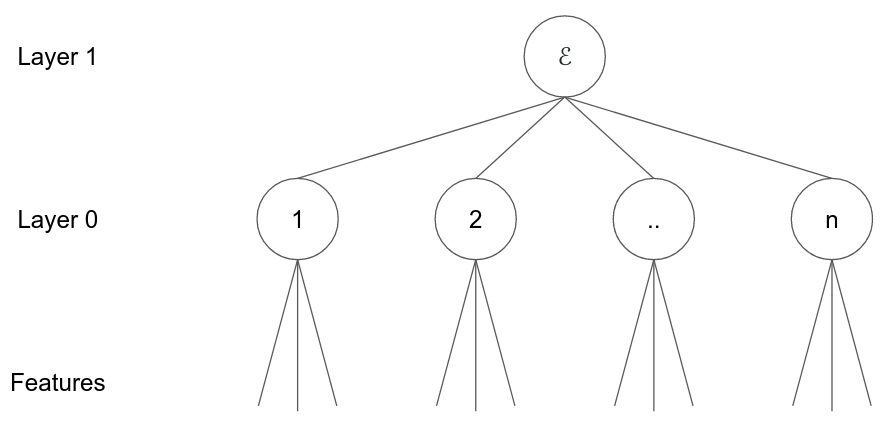
\includegraphics[width=0.8\textwidth]{Figures/dia_multilayer.png}
	\caption{Multi layer model representation.}
	\label{fig:dia_multilayer}
\end{figure}

%%%%%%%%%%%%%%%%%%%%%%%%%%%%%%%%%%%%%%%%%%%%%%%%%%%%%%%%%%%%%%%%%%%%%%%%
\subsection{Malware Classes}

With this new model defined, we now present our approach on selecting the $n$ classes of interest.
This represents another labeling problem, but now instead of having to label between goodware and malware, we have to label the malware as belonging to some subclass.

To choose the malware classes for our datasets, we take into account our description in Chapter \ref{chapter:related_work} regarding propagation methods and malware names based on purpose.
With this in mind, we chose 6 malware classes: \textit{virus}, \textit{trojan}, \textit{worm}, \textit{ransom}, \textit{spyware} and \textit{other}.
The first three classes, \textit{virus}, \textit{trojan} and \textit{worm}, were chosen from the propagation methods, whereas \textit{ransom} and \textit{spyware}
where chosen due to their popularity in recent years. The last class, \textit{other}, serves for any malware that does not fit the previous five.

As mentioned in Chapter \ref{chapter:related_work}, there is no agreed upon naming convention for malware, which translates into different names for the same malware sample.
To minimize this problem, we referenced a tool by Sebastián, M. et al.~\cite{sebastian2016avclass}, AVClass, which was built to normalize a malware sample name into the most likely family, using the names provided by VirusTotal~\cite{tool:virustotal}.

We took advantage of this tool and modified it such that instead of providing a family name, it would provide one (or more) of the 6 previously defined classes.
Specifically, we changed it in a way that given a set of malware names, the output would be a distribution over the 6 malware classes.

To calculate each class weight we apply the following formula
\begin{eqnarray*}
	\mathcal{W}_c = \dfrac{f_c}{\sum\limits_{c}f_c}
\end{eqnarray*}

where $f_c$ is the frequency for the class $c$ and $\sum_{c}f_c$ is the number of times all classes appear.
For example, if a given set of names contain the name \textit{trojan} 3 times and the name \textit{virus} one time, then the weights would be
\begin{eqnarray*}
	\mathcal{W}_{trojan}=\dfrac{3}{4}=0.75,~\mathcal{W}_{virus}=\dfrac{1}{4}=0.25,~ \mathcal{W}_{c}=0, c \in \{worm, spyware, other, ransom\}
\end{eqnarray*}

\medskip

Having these malware classes defined for our multi layer model, we also added the \textit{goodware} class for samples that are not malware.
Doing so gives us 7 possible classes, 6 of which are malware only.
It is worth mentioning that if a sample belongs to the \textit{goodware} class, it cannot belong to any other, likewise, if it belongs to any malware class, it cannot belong to the \textit{goodware} class.

By applying this new labeling, we refine our previous datasets $\CC_{strict}$, $\CC_{loose}$ and $\CC_{real}$ as shown in Table \ref{tab:dataset_sizes_new}.

\begin{table}[!htb]
	\renewcommand{\arraystretch}{1.2} % more space between rows
	\centering
	\begin{tabular}{lccc}
		\toprule
		Dataset			& $\CC_{real}$ & $\CC_{loose}$ & $\CC_{strict}$	\\
		\midrule
		Trojan			& 0 & 0 & 0\\
		Virus			& 0 & 0 & 0\\
		Worm			& 0 & 0 & 0\\
		Spyware			& 0 & 0 & 0\\
		Ransom			& 0 & 0 & 0\\
		Other			& 0 & 0 & 0\\
		\midrule
		Total Malware	& 0 & 0 & 0\\
		Total Goodware	& 0 & 0 & 0\\
		\midrule
		\midrule
		Total			& 0 & 0 & 0\\
		\bottomrule
	\end{tabular}
	\caption{New sizes for datasets $\CC_{real}$, $\CC_{loose}$ and $\CC_{strict}$.}
	\label{tab:dataset_sizes_new}
\end{table}

In sum, we added a layer of labeling to our dataset, where a sample can either belong to the \textit{goodware} class, or to a set of the other 6 malware classes.
This concludes the description of our first improvement to the model, what follows are our improvements regarding features.

%%%%%%%%%%%%%%%%%%%%%%%%%%%%%%%%%%%%%%%%%%%%%%%%%%%%%%%%%%%%%%%%%%%%%%%%
\section{Dynamic Features}
\label{section:improvements_dynamic_features}

Having described our first model improvement, we now proceed to our second enhancement, which takes advantage of the amount of information available in Cuckoo's~\cite{tool:cuckoo} reports.

In the previous chapter, we used static imports as features for our malware detection model.
Although the results are reasonable, the information which can be retrieved from static imports alone is limited.
As an example, if a sample is compressed, encrypted or packed, its behavior cannot be inferred from static imports only.
To overcome these limitations, we resort to more dynamic information provided by Cuckoo.

Given that Cuckoo runs the provided samples inside a virtual machine, it monitors the sample from a dynamic point of view.
This monitoring includes information like the sequence of library calls and their categories and network and file activity.
With this in mind, we now detail what dynamic information we extracted from the reports.

%%%%%%%%%%%%%%%%%%%%%%%%%%%%%%%%%%%%%%%%%%%%%%%%%%%%%%%%%%%%%%%%%%%%%%%%
\subsection{Category Calls}
\label{section:improvements_categories}

The first type of dynamic information we extracted were the number of dynamic category calls.
When Cuckoo runs and monitors a sample, it registers some low level library calls, which it then assigns to a fixed number of categories.

There are a total of 14 different categories defined by Cuckoo: \textit{anomaly}, \textit{device}, \textit{filesystem}, \textit{hooking}, \textit{misc}, \textit{network}, \textit{process}, \textit{registry}, \textit{services}, \textit{socket}, \textit{synchronization}, \textit{system}, \textit{threading} and \textit{windows}.
After using Celery~\cite{tool:celery} to extract the number of each category calls for the samples, we obtained a total of 148,036 samples with information regarding category calls.

Figure \ref{fig:boxplot_category_calls} shows a boxplot for the category calls, where one can see the categories \textit{filesystem}, \textit{registry} and \textit{system} are the ones with higher mean, hence more used than the other categories.
Although not depicted, some outliers for the number of category calls go up to 1,400,000, which do not provide useful information other than the number of category calls is very high.

\begin{figure}[!htb]
	\centering
	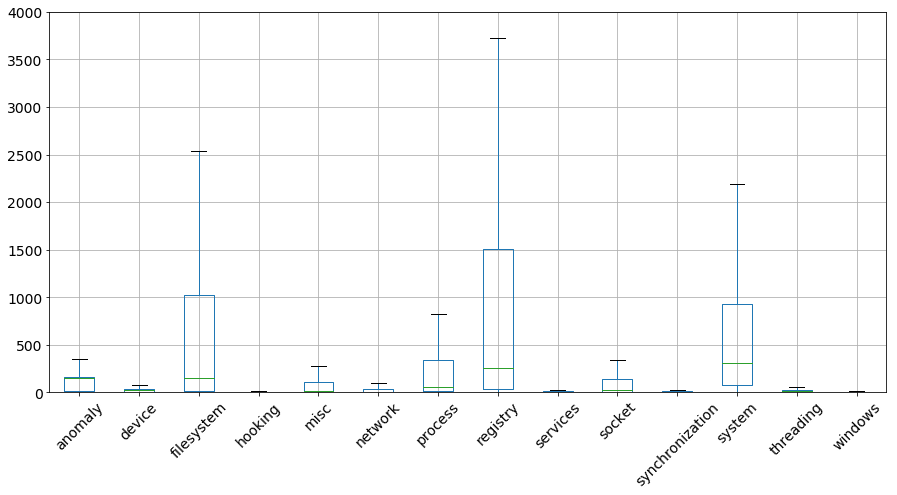
\includegraphics[width=\textwidth]{Figures/boxplot_category_calls.png}
	\caption{Category calls boxplot.}
	\label{fig:boxplot_category_calls}
\end{figure}

With that in mind, we decide to transform the values into a $[0,1]$ range.
We do this by using scikit-learn's~\cite{tool:sklearn} \textit{QuantileTransformer} with a normal distribution, which splits the possible values into bins such that the resulting distribution is of type \textit{Gaussian} with a mean of 0.
This way we have a greater number of bins around the mean, allowing for better discrimination, whereas very large values fall into the same bin.

%%%%%%%%%%%%%%%%%%%%%%%%%%%%%%%%%%%%%%%%%%%%%%%%%%%%%%%%%%%%%%%%%%%%%%%%
\subsection{Library Calls}
\label{section:improvements_api_unigrams}

Our second type of dynamic information are the number of library calls, which closely relate to the previous feature.
While \textit{category calls} provide the number of calls for a given category, \textit{library calls} provide the count for each library call, hence being a subset of the previous.

Cuckoo~\cite{tool:cuckoo} registers the number of calls for 163 different functions, ranging from opening and closing files, to opening and closing sockets.
Again we used Celery~\cite{tool:celery} to extract these numbers, obtaining information from 148,036 samples.

Given we are dealing with a high number of features (163 different library calls), we decided to apply the same variance threshold as in Section \ref{section:feature_selection}, to remove features that do not vary in most samples.
By choosing a threshold of 80\%, we remove library calls that do not vary in more than 80\% of the samples, effectively reducing the number of library calls to 144.
With regards to how these features can vary from 0 to $+\infty$, as before, we again apply a quantile transformer with a normal distribution.

%%%%%%%%%%%%%%%%%%%%%%%%%%%%%%%%%%%%%%%%%%%%%%%%%%%%%%%%%%%%%%%%%%%%%%%%
\subsection{Cuckoo Signatures}
\label{section:improvements_categories}

For our third and last type of dynamic information, we resort to Cuckoo~\cite{tool:cuckoo} custom signatures.
These signatures are built from certain activities that Cuckoo deems malicious or suspicious.
For example, if a sample allocates memory and then makes it executable, it might suggest some sort of packing or obfuscation.

Although some signatures are defined by a sequence of library calls, which could also be attained by creating n-grams of our previously defined feature, using the already defined Cuckoo signatures saves training time.
As an example, creating bi-grams of library calls, given there are 144 unique calls, would yield over 20,000 possible features, hence being unpractical.

To extract these signatures, we use Celery~\cite{tool:celery} and obtain a total of 124,821 samples and 61 different signatures.
As with our static import features, we use a binary vector for each sample, where each position corresponds to a specific signature. Re-iterating on how we represent this, if a given signature $i$ is present in a sample, its feature vector $x$ will have the value 1 at that position $x_i$. Likewise, if a given signature $j$ is not present in a sample, its feature vector $x$ will have the value 0 at that position $x_j$.

\medskip

Having these new features, we create a new set with all features (static, category and library calls and signatures) $\FF_{dynamic}$.
We joined these samples $\FF_{dynamic}$ to the labeled samples $\CC_{real}$, obtaining a total of \miss{size} labeled samples with dynamic imports $\DD_{dynamic} = \CC_{real} \cap \FF_{dynamic}$.

% To reduce the number of features into those that are more representative, we apply, as in other features, a variance threshold, removing signatures that do not vary in more than 80\% of the samples.
% By doing so, we reduce the total number of signatures to 

%%%%%%%%%%%%%%%%%%%%%%%%%%%%%%%%%%%%%%%%%%%%%%%%%%%%%%%%%%%%%%%%%%%%%%%%
\section{Improved Model Results}
\label{section:improvements_results}

In the previous sections we described all our modifications to the original model $\LR$: a two layer approach that splits malware into subclasses and the addition of three dynamic features.
We now present the results of our new model $\mathcal{E}$, validated using the same methodology as described in \ref{section:evaluation}.
Specifically we test the model using the baseline cross-validation methodology, followed by our three temporally consistent scenarios: \textit{Past-to-Present}, \textit{Present-to-Past} and \textit{Temporal Window}.
We test each methodology using the three different scenarios: $\mathcal{S}_{\strict}$, $\mathcal{S}_{\loose}$ and $\mathcal{S}_{\real}$.

We again use the resources provided by INOV - Inesc Inovação, together with scikit-learn~\cite{tool:sklearn}, Pandas~\cite{tool:pandas} and Jupyter Interactive Notebooks~\cite{tool:jupyter} to train and analyze the data.

\medskip

Starting with \textit{laboratory conditions}, we apply the cross-validation evaluation to model $\mathcal{E}$ with the labeled dataset $\CC_{strict}$ and features $\DD_{dynamic}$, providing scenario $\mathcal{S}_{\strict}$.
For this scenario, we obtain an \gls{auroc} of \miss{score}, as presented by the red line in Figure \ref{fig:improved_xval}.
These provide the highest results, provided by factors like a small and reliable dataset, more features and the use of cross-validation.

Relaxing to more \textit{real-world conditions}, under the form of a less reliable ground truth, we test the datasets $\CC_{loose}$ and $\CC_{real}$ on features $\DD_{dynamic}$.
As shown in Figure \ref{fig:improved_xval}, the score under \gls{auroc} decreases to \miss{socre} for $\mathcal{S}_{\loose}$ (blue line) and \miss{score} for $\mathcal{S}_{\real}$ (green line).

\begin{figure}[!h]
	\centering
	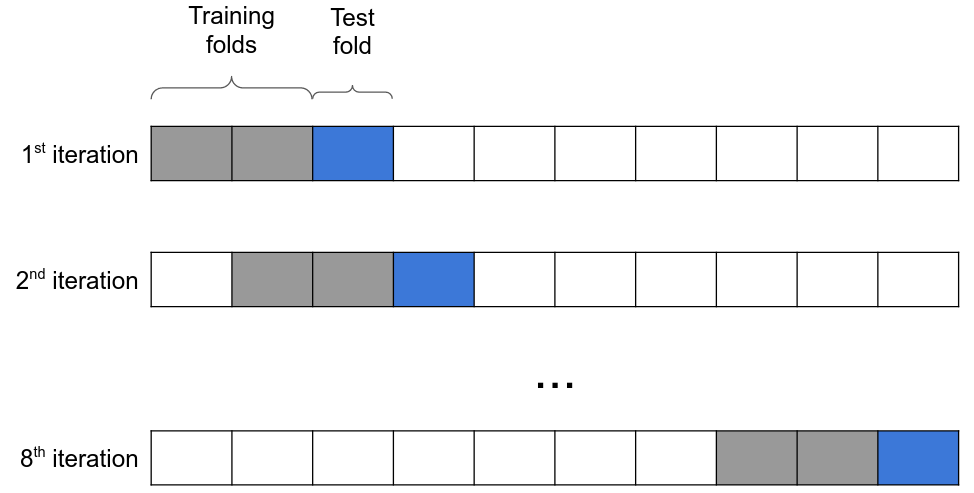
\includegraphics[width=0.8\textwidth]{Figures/dia_slidingwindow.png}
	\caption{Improved model results with dynamic features in laboratory conditions.}
	\label{fig:improved_xval}
\end{figure}

% Adicionar seccao para resultados do multi layer apenas.

As with previous results, one notes that from $\mathcal{S}_{\strict}$ to $\mathcal{S}_{\loose}$ the results are not highly affected, when the change between the scenarios is merely in the number of malware samples.

Between $\mathcal{S}_{\loose}$ to $\mathcal{S}_{\real}$ we again note the already seen pattern, the lowest score when using the most realistic dataset.

\todo[inline]{}

When looking at the changes from $\mathcal{S}_{\loose}$ to $\mathcal{S}_{\real}$, not only the amount of malware labeled samples increase, but also the number of goodware labeled samples, both by a significant amount. 
The way this impacts the results is pretty significant, as we observe a high decrease in the \gls{auroc} for both models.
The metric $\Mrealv$ that labels malware and goodware for this scenario $\mathcal{S}_{\real}$ disregards the cross-check from outside repositories, which in turn degrade the reliability significantly, as well as increase the dataset size notably.
We attribute the results' degradation mainly to the unreliability of goodware labeling, not only because we have previously seen that increase in malware does not significantly impact results (from $\mathcal{S}_{\strict}$ to $\mathcal{S}_{\loose}$), but also due to the tendency for false negatives in vendors (Figure \ref{fig:dups_frequency}), which in turn lead us to incorrectly label goodware for the samples in $\CC_{real}$.

The results we described show how relaxing \textit{laboratory conditions} to more \textit{real-world conditions} degrade the model's performance.
We now focus on using our previously defined temporal based methodologies to further converge into a real-world scenario.

\medskip

We start by applying our \textit{Past-to-Present} validation to the three scenarios, $\mathcal{S}_{\strict}$, $\mathcal{S}_{\loose}$ and $\mathcal{S}_{\real}$.
As previously defined, this validation starts with an older set of training samples and iteratively adds newer samples, validating each iteration on a fixed set of the most recent samples.
Since our interest is to measure performance variation over time, we plot in Figure~\ref{fig:pastpresent} the \gls{auroc} at every iteration (\ie, fold), for each of our three scenarios.

\begin{figure}[!htb]
	\centering
	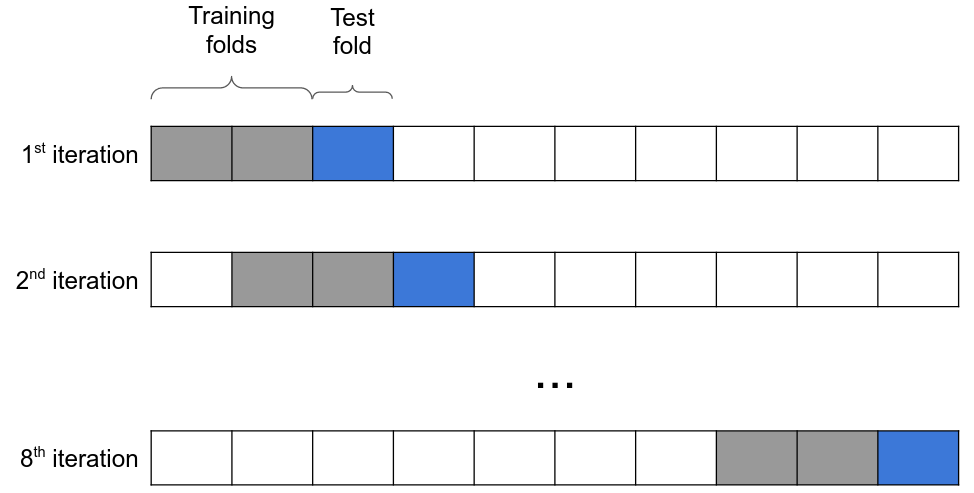
\includegraphics[width=0.8\textwidth]{Figures/dia_slidingwindow.png}
	\caption[Single layer results for static features in \textit{Past-to-Present}.]{\gls{auroc} for each iteration of the \textit{Past-to-Present} evaluation. Folds order consistent with temporal order (\ie\ fold 0 contains older samples than
		fold 1)}
	\label{fig:pastpresent}
\end{figure}

When directly comparing the average \gls{auroc} for cross-validation and our \textit{Past-to-Present} validation, we note a decrease from \miss{score} to \miss{score} for $\mathcal{S}_{\strict}$, \miss{score} to \miss{score} for $\mathcal{S}_{\loose}$, and \miss{score} to \miss{score} for $\mathcal{S}_{\real}$.
This decrease is intuitive to the methodology, as we are forcing temporal consistency between samples.

When looking at results from $\mathcal{S}_{\strict}$ and $\mathcal{S}_{\loose}$, we see they closely relate.
This relation has already been noticed on previous cross-validation results, as their metrics $\Mstrictv$ and $\Mloosev$ are not very different.
As for $\mathcal{S}_{\real}$, the degradation is higher, as the reliability of the metric $\Mrealv$ goes down.

Our main observation for this validation methodology is that there is a slight tendency for \gls{auroc} to increase, as we move forward in time, close to the validation set.

Both $\mathcal{S}_{\strict}$ and $\mathcal{S}_{\loose}$ behave similarly under our \textit{Past-to-Present} evaluation, decreasing the \gls{auroc} until fold \miss{fold}, after which both increase, stabilizing around \miss{score} \gls{auroc} by the last \miss{two} folds. As for $\mathcal{S}_{\real}$, its \gls{auroc} does not vary significantly, although a subtle increase over time is noticeable.

\medskip

Our next result, which uses our \textit{Present-to-Past} validation methodology will further help analyze the aforementioned detail.
The \textit{Present-to-Past} validation enhances the previous results under real-world conditions.
This methodology starts by fixing the validation set to the most recent samples, but with the training set starting at the temporally closest samples to validation.
At each iteration, older samples are added to the training set and validated on the fixed, most recent, samples.

By applying this methodology to the three scenarios, $\mathcal{S}_{\strict}$, $\mathcal{S}_{\loose}$ and $\mathcal{S}_{\real}$, we plot Figure \ref{fig:presentpast}, where the X axis increases as older samples are added to the training set (\ie\ fold 0 contains newer samples than fold 1), hence measuring the performance variance over time.
Similarly to the previous observation, the average \gls{auroc} suffers a decrease when compared to cross-validation. For $\mathcal{S}_{\strict}$ we note a change from \miss{score} to \miss{score}, for $\mathcal{S}_{\loose}$ the decrease is from \miss{score} to \miss{score}, and for $\mathcal{S}_{\real}$ \miss{score} to \miss{score}.

\begin{figure}[!h]
	\centering
	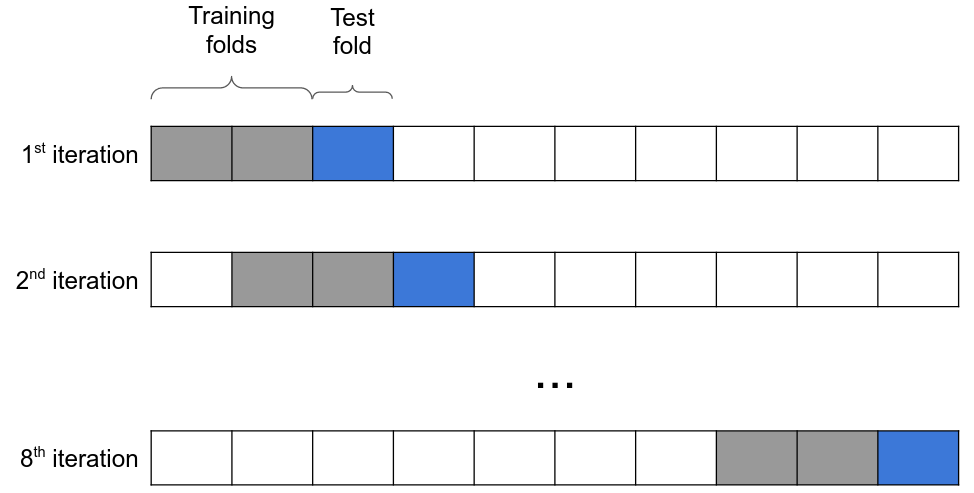
\includegraphics[width=0.8\textwidth]{Figures/dia_slidingwindow.png}
	\caption[Single layer results for static features in \textit{Present-to-Past}.]{\gls{auroc} for each iteration of the \textit{Present-to-Past} evaluation. Folds order is the inverse of temporal order (\ie\ fold 0 contains newer samples than fold 1)}
	\label{fig:presentpast}
\end{figure}

The comparison between scenarios is identical to what was observed in cross-validation and \textit{Past-to-Present}: scenarios $\mathcal{S}_{\strict}$ and $\mathcal{S}_{\loose}$ display very similar results, with $\mathcal{S}_{\real}$ dropping behind due to its less reliable labeling metric.

With these results, our original observation that samples closer to the validation set benefit the model becomes more convincing. In fact, we argue that there should be an ideal number of necessary training folds, temporally consistent with the validation fold (\ie\ any fold from training predates validation), needed to maximize the overall score.

\medskip

Finally, we analyze how does such reduced training set behaves in our scenarios; for this purpose, we define a sliding window that moves forward in time through each scenario for training and validation.
We propose a reduction on the training size to \miss{$w=3$} folds predating the validation fold. We choose \miss{$w = 3$}, since we have seen that the scores either do not improve (for $\mathcal{S}_{\strict}$ and $\mathcal{S}_{\loose}$) or actually go down (for $\mathcal{S}_{\real}$) with higher folds.
In summary, we have selected \miss{30\%} of each dataset for training purposes and the next \miss{10\%} for validation \miss{(3 training folds, 1 validation fold)}, and then started moving the window forward in time (1 fold at a time) to obtain the following results (Figure~\ref{fig:slidingwindow}): for  $\mathcal{S}_{\strict}$, $\mathcal{S}_{\loose}$ and $\mathcal{S}_{\real}$, we obtain \gls{auroc} values of \miss{score, score and score}, respectively. 
These results come to reaffirm our argument that we can reduce the size of the training set, without losing any significant score.

\begin{figure}[!h]
	\centering
	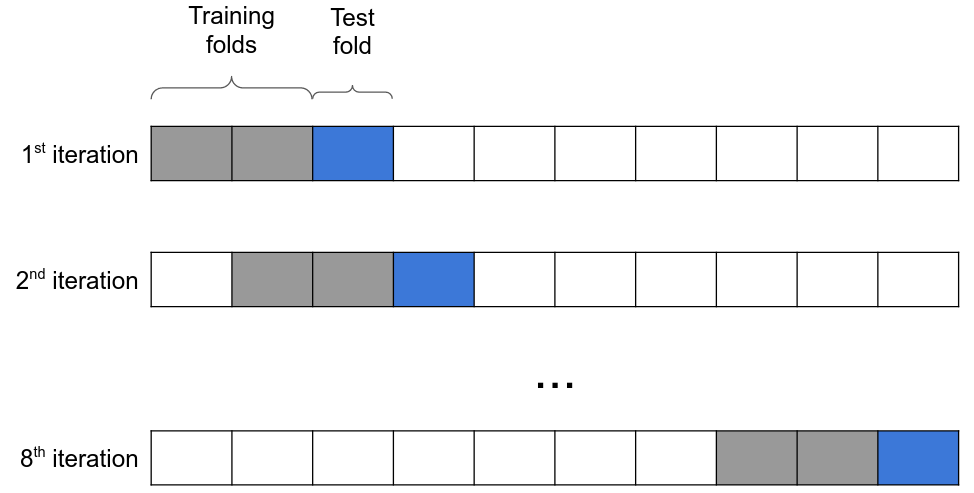
\includegraphics[width=0.8\textwidth]{Figures/dia_slidingwindow.png}
	\caption[Single layer results for static features in \textit{Temporal Window}.]{\gls{auroc} for our three scenarios, under the \textit{Temporal Window} methodology.}
	\label{fig:slidingwindow3}
\end{figure}

Comparing these results with the baseline cross-validation, we note a decrease for each scenario, specifically a decrease from \miss{0.93 to 0.87 for $\mathcal{S}_{\strict}$, from 0.92 to 0.86 for $\mathcal{S}_{\loose}$ and from 0.79 to 0.76 for $\mathcal{S}_{\real}$.}
We should highlight that the results that use temporal-consistency should better reflect the reality than standard cross-validation, since we are requiring temporal consistency.
Another important idea that should be stressed is that for cross validation we used a fairly reasonable amount of data for training purposes, whereas in this last case we used a restricted amount of data. This might be a relevant issue in a few year's time. The results obtained are summarized in Table \ref{tab:multilayer_results}.

\begin{table}[!htb]
	\renewcommand{\arraystretch}{1.2} % more space between rows
	\centering
	\begin{tabular}{ccccc}
		\hline AUROC & $\DS_\strict$ & $\DS_\loose$ & $\DS_\real$ & Train/Test \%\\
		\hline Cross-Validation & 0.93 & 0.92 & 0.79 & 90 / 10\\
		\hline Past-to-Present & 0.88 & 0.87 & 0.71 & 10 to 90 / 10\\
		\hline Present-to-Past & 0.90 & 0.86 & 0.72 & 10 to 90 / 10\\
		\hline Sliding-Window & 0.87 & 0.86 & 0.76 & 30 / 10\\
		\hline
	\end{tabular}
	\caption{Single layer results summary.}
	\label{tab:multilayer_results}
\end{table}
